\documentclass[tikz]{standalone}

\usepackage[utf8]{inputenc}
\usepackage[T1]{fontenc}
\usepackage{cmap}
\usepackage{amsmath}
\usepackage{amssymb}
\usepackage{verbatim}
\usepackage{bm}
\usepackage{siunitx}

\renewcommand{\familydefault}{\sfdefault}
\usepackage[cm]{sfmath}

\usepackage{tikz}
\usetikzlibrary{math}
\usetikzlibrary{bending}
\usetikzlibrary{decorations.pathreplacing}
\usetikzlibrary{decorations.pathmorphing}
\usetikzlibrary{fadings}
\usetikzlibrary{positioning}
\definecolor{cblue}{rgb}{0.396, 0.643, 0.82}
\definecolor{corange}{rgb}{1.0, 0.69, 0.416}
\definecolor{cgreen}{rgb}{0.471, 0.824, 0.471}
\definecolor{cred}{rgb}{1.0, 0.502, 0.502}
\definecolor{cpurple}{rgb}{0.863, 0.78, 0.937}

\def\symbhwaas{N_a}
\def\symbsteplen{\Delta d}
\def\symbsweeprate{f_s}
\def\symbsweepperiod{T_s}
\def\symbsweepdur{\tau_s}
\def\symbframerate{f_f}
\def\symbframeperiod{T_f}
\def\symbframedur{\tau_f}
\def\symbprf{f_\text{p}}
\def\symbspf{N_s}
\def\symbstartpoint{d_1}
\def\symbnumpoints{N_d}
\def\symbmur{r_\text{u}}
\def\symbcid{r_\ell}
\def\symbminmd{r_\text{min}}
\def\symbmaxmd{r_\text{max}}
\def\symbdcrnear{r_\text{near}}
\def\symbdcrfar{r_\text{far}}

\begin{document}

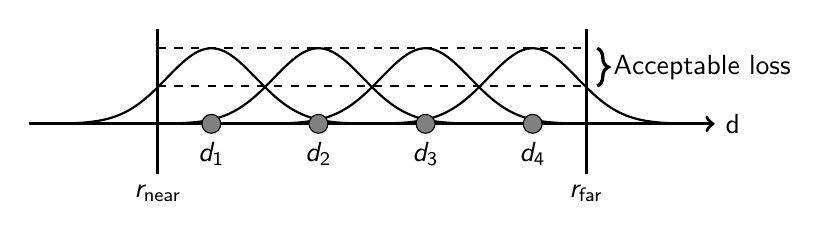
\begin{tikzpicture}[scale=0.8]
  \tikzmath{
    \sx = 1.7;
    \nump = 4;
  }

  % axis
  \draw [very thick, ->] (-1.2*\sx, 0) -- ({(\nump+1.2)*\sx}, 0) node[right]{d};
  \draw [very thick] (0, 0) ++(0, 1.5) -- ++(0, -2.3) node[below]{$\symbdcrnear$};
  \draw [very thick] ({\nump*\sx}, 0) ++(0, 1.5) -- ++(0, -2.3) node[below]{$\symbdcrfar$};

  \foreach \i in {1, ..., \nump} {
    \tikzmath{
      \xc = (\i-0.5)*\sx;
    }
    \draw [thick, domain=-2.5:2.5, smooth, samples=50, variable=\x, shift={(\xc, 0)}]
    plot (\x, {1.2*exp(-(\x)^2)});
  }
  \draw [thick, dashed] (0, 0.6) -- ++(\nump*\sx, 0);
  \draw [thick, dashed] (0, 1.2) -- ++(\nump*\sx, 0);
  \draw [very thick, decoration={brace, amplitude=4pt, raise=4pt}, decorate] (\nump*\sx, 1.2) -- node[right=6pt] {Acceptable loss} ++(0, -0.6);

  \foreach \i in {1, ..., \nump} {
    \tikzmath{
      \xc = (\i-0.5)*\sx;
    }
    \draw [fill=gray] (\xc, 0) circle (1.5mm) node[below=3pt]{$d_\i$};
  }
\end{tikzpicture}

\end{document}
